\section{IBD selection}

Two independent IBD selection criteria have been developed by IHEP (A1) and SYSU (A2). Both selections follow the same logic: the delayed signal is identified first, followed by a search for the corresponding prompt signal. The main differences lie in the definitions of the muon veto windows and the multiplicity cut. Results are consistent between the two groups.
%Both apply similar prompt–delayed energy, time, and distance cuts. The selection A2 adopts slightly different muon veto windows and broader spallation neutron veto ($\Delta r <$ 3 m, $\Delta t <$ 1.6 s) than the A1 version. 
More details are presented below.

\subsection{Selection A1}

\subsubsection{Data preparation} 
    We have applied vetoes based on muons and spallation neutrons in the bad files, as described below. As an alternative approach, one may first remove the bad esd files and then apply a 1.2 s veto after each time gap. This alternative strategy has been tested and found to produce consistent results. We therefore employ the former strategy, which offers higher signal efficiency.
    \begin{enumerate}
        \item Based on mini-ESD produced by merging all files in good runs.
        \item Both good files and bad files are included in mini-ESD. The contribution of the bad files to IBD candidates and efficiency estimation will be removed. But the veto is performed as nomal based on the muons and spallation neutrons from bad files. 
        \item Split files into jobs: split at the end of a run or if the number of files reaches 10 in one job. Veto the first 1.2~s for each job.
        \item We use bad time list prepared by DQ group to remove IBD candidates in bad files. 
    \end{enumerate}
    \subsubsection{Event selection} 
    \begin{enumerate}
        \item Disordering processing: if the current event is CD event and earlier than the previous CD event, record and skip.
        \item Muon identification: CD event with $Q>3 \times 10^4$ PE or WP event with $Q>700$ PE. 
        %We also treat the first event of a job as a fake muon. 
        If the current event is a muon, skip this event.
        \item Spallation neutron identification:
        \begin{enumerate}
            \item Time to the last CD muon: 20~$\mu$s $< dt < $2~ms.
            \item Spallation neutron charge: 3000 < Q < 30000 PE.
        \end{enumerate}
        \item Find a delayed signal candidate:
        \begin{enumerate}
            \item CD event.
            \item Delayed energy cut: 2.0 < E < 2.5 MeV.
            \item Veto the beginning of job with $T_{veto} = 1.2$~s.
            \item Muon veto with $T_{veto} = 5$~ms.
            \item Spallation neutron veto with  $T_{spnVeto} = 1.2$~s and $R_{spnVeto} = 4$~m.
        \end{enumerate}
        \item Paring: find prompt signal before the current event.
        \begin{enumerate}
            \item Prompt signal.
            \begin{enumerate}
                \item CD event passing FV cut.
                \item Energy cut: $0.7 < E_p < 12 $~MeV.
            \end{enumerate}
            \item Correlation time window: $5\mu s<T_{corr} < 1 ms$.
            \item Distance cut: $D_{max} = 1.5 m$
        \end{enumerate}
        \item Multiplicity cut: no third event before and after the delayed signal candidate.
        \begin{enumerate}
            \item Definition of the third event:
            \begin{enumerate}
                \item CD event in the FV with energy >0.7~MeV.
                \item or CD event outside the FV with energy [2.0, 2.5]~MeV.
            \end{enumerate}
            \item Multiplicity time window: $2 \times T_{corr}$ before the delayed signal, and $T_{corr}$ after.
            \item If a muon is found in the multiplicity time window, let the event pair pass multiplicity cut.
        \end{enumerate}
    \end{enumerate}
    \subsubsection{Post-processing} 
    \begin{enumerate}
        \item Remove event pairs including an event from bad files.
        \item Calculation of DAQ time. $T_{DAQ} =  t_{last} - t_{first} - T_{bad files}$
     %   \item Remove event pairs with $dt < 5 \mu s$
    \end{enumerate}


\subsection{Selection A2}

The general IBD selection strategy of selection A2 is very similar to A1 except the following:

\begin{itemize}
    \item CD muon veto: each CD muon (nPE > 3$\times 10^4$) vetoes the whole CD 7 ms ([-1 ms, 6 ms] relative to the delayed signal)
    \item WP muon veto: each WP muon (nPE > 700) vetoes the whole CD 2 ms ([-2 $\mu$s, 2 ms] relative to the delayed signal)
    \item muon spallation neutron (spn): any CD events (1.8 MeV $< E_{\rm rec} < $ 10 MeV) after the muon within [50 $\mu$s, 1 ms]
    \item multiplicity cut: No other event (0.7 MeV $< E_{\rm rec} < $ 15 MeV) are allowed at [-2 ms, 1 ms] time window relative to the delayed signal except its intrinsic prompt signal
\end{itemize}

The multiplicity cut is mainly to remove strange continuous triggers and any ambiguity pairs. The spn veto is mainly to reduce $^{9}$Li cosmogenic muon isotopes which are usually associated with spn neutrons. More detailed information can check with DocDB-14948. 

Figure~\ref{fig:muon_rate} shows the muons as defined here as a function of time.

\begin{figure}[!htbp]
    \centering
    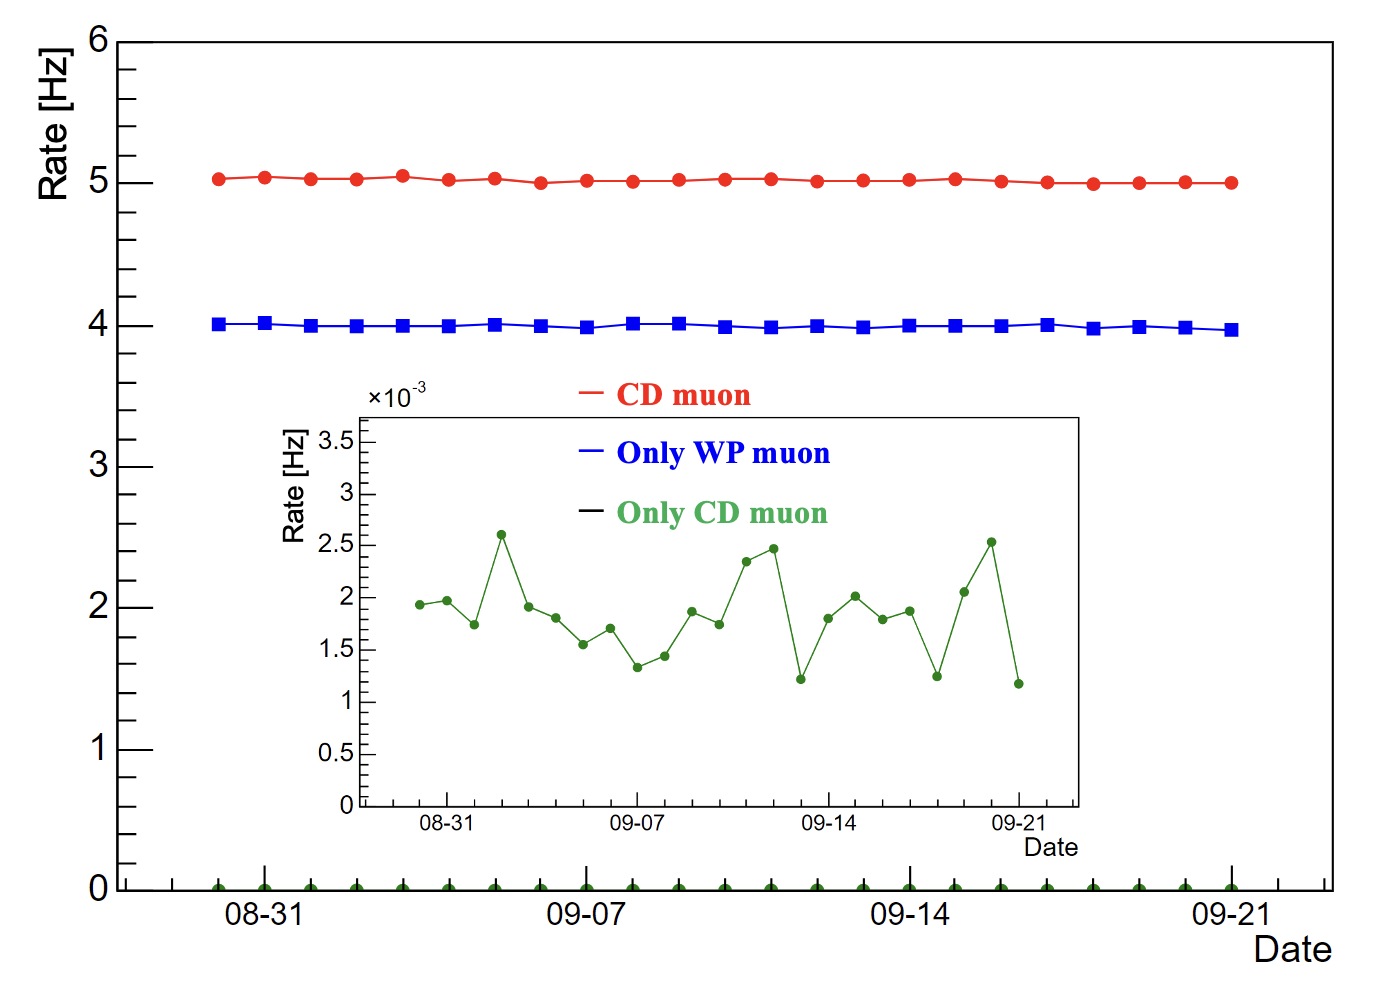
\includegraphics[width=10cm]{2_selection/muon_rate.png}
    \caption{Muon rate as a function of time.}
    \label{fig:muon_rate}
\end{figure}

\subsection{Summary}


Table~\ref{tab:ibd_selection} shows the summary of IBD selection criteria from two groups.
\begin{table}[!htbp]
    \caption{Summary of IBD selection criteria.}
    \label{tab:IbdSel}
    \centering
    \footnotesize% fontsize
    \setlength{\tabcolsep}{4pt}% column separation
    \renewcommand{\arraystretch}{1.2}%row space 
    %\resizebox{\linewidth}{!}{
    \begin{tabular}{lm{6cm}m{6cm}}
        \hline
        Criterion & Selection A1 (IHEP) & Selection A2 (SYSU) \\ 
        \hline
        PMT flasher & Applied & - \\
        %Fiducial volume & \multicolumn{2}{c}{r < 16.5 m, |z| < 15 m} \\
        Fiducial volume & r < 16.5 m, |z|<15.5m & r < 16.9 m, |z|<15.5m \\
        Prompt energy  & (0.7, 12) MeV & [0.7, 12] MeV \\
        Delayed energy & (2.0, 2.5) MeV & [2.0, 2.5] MeV\\
        Coincidence time & (5, 1000) $\mu$s & [5, 1000] $\mu$s \\
        Relative distance & < 1.5 m & < 1.5 m \\
        Multiplicity cut & No other events > 0.7~MeV in the FV or (2.0, 2.5)~MeV outside the FV within 2 ms before  and 1 ms after the delayed & No other events with energy (0.7, 15) MeV in the FV within 2 ms before the delay or within 1 ms after delay \\
        Water pool muon veto & Veto if the delayed is within (0, 5 ms) after NPE > 700 in WP & Veto [-2 $\mu$s, 2 ms] after NPE > 700 in WP \\
        CD muon veto & Veto if the delayed is within (0, 5 ms) after NPE > $3 \times 10^{4}$ in CD & Veto [-1 ms, 6.0 ms] after NPE > $3 \times 10^{4}$ in CD \\
        Spallation neutron veto & Veto if the delayed satisfies $\Delta r$ < 4 m and $\Delta t$ < 1.2 s after spallation neutrons with NPE$_{spn} \in$ (3000, 30000) and $T_{spn2\mu} \in$ (20, 2000) $\mu$s & Veto $\Delta r$ < 4 m and $\Delta t$ < 1.2 s after spallation neutrons  with $E_{spn} \in$ (1.8, 10) MeV and $T_{spn2\mu} \in$ (50, 1000) $\mu$s \\
        \hline
    \end{tabular}
    %}
    \label{tab:ibd_selection}
\end{table}

Figures~\ref{fig:IBD_energy_spectra}, \ref{fig:IBD_energy_spectra_2D}, \ref{fig:IBD_dt}, \ref{fig:IBD_r3} and \ref{fig:IBD_vertex} show the distributions of the selected IBD candidates. Figure~\ref{fig:IBDrate} shows the raw IBD rate as a function of time.

\begin{figure}[!htbp]
    \centering
      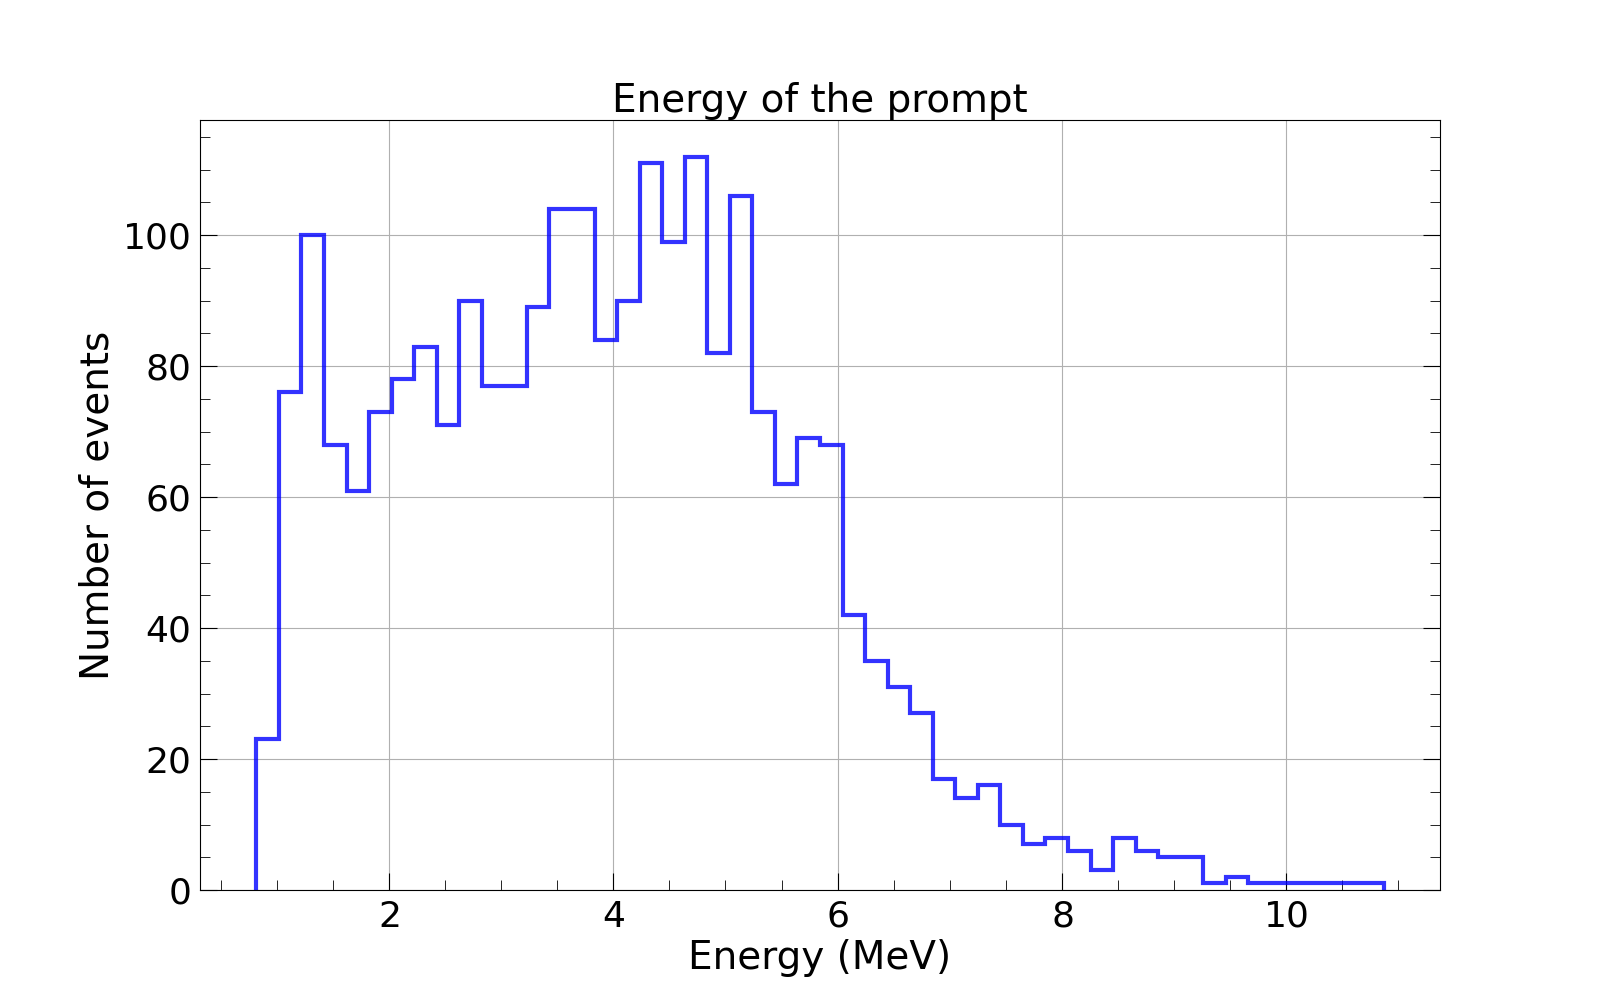
\includegraphics[width=0.49\textwidth]{2_selection/h_ibd_e_p.png}
      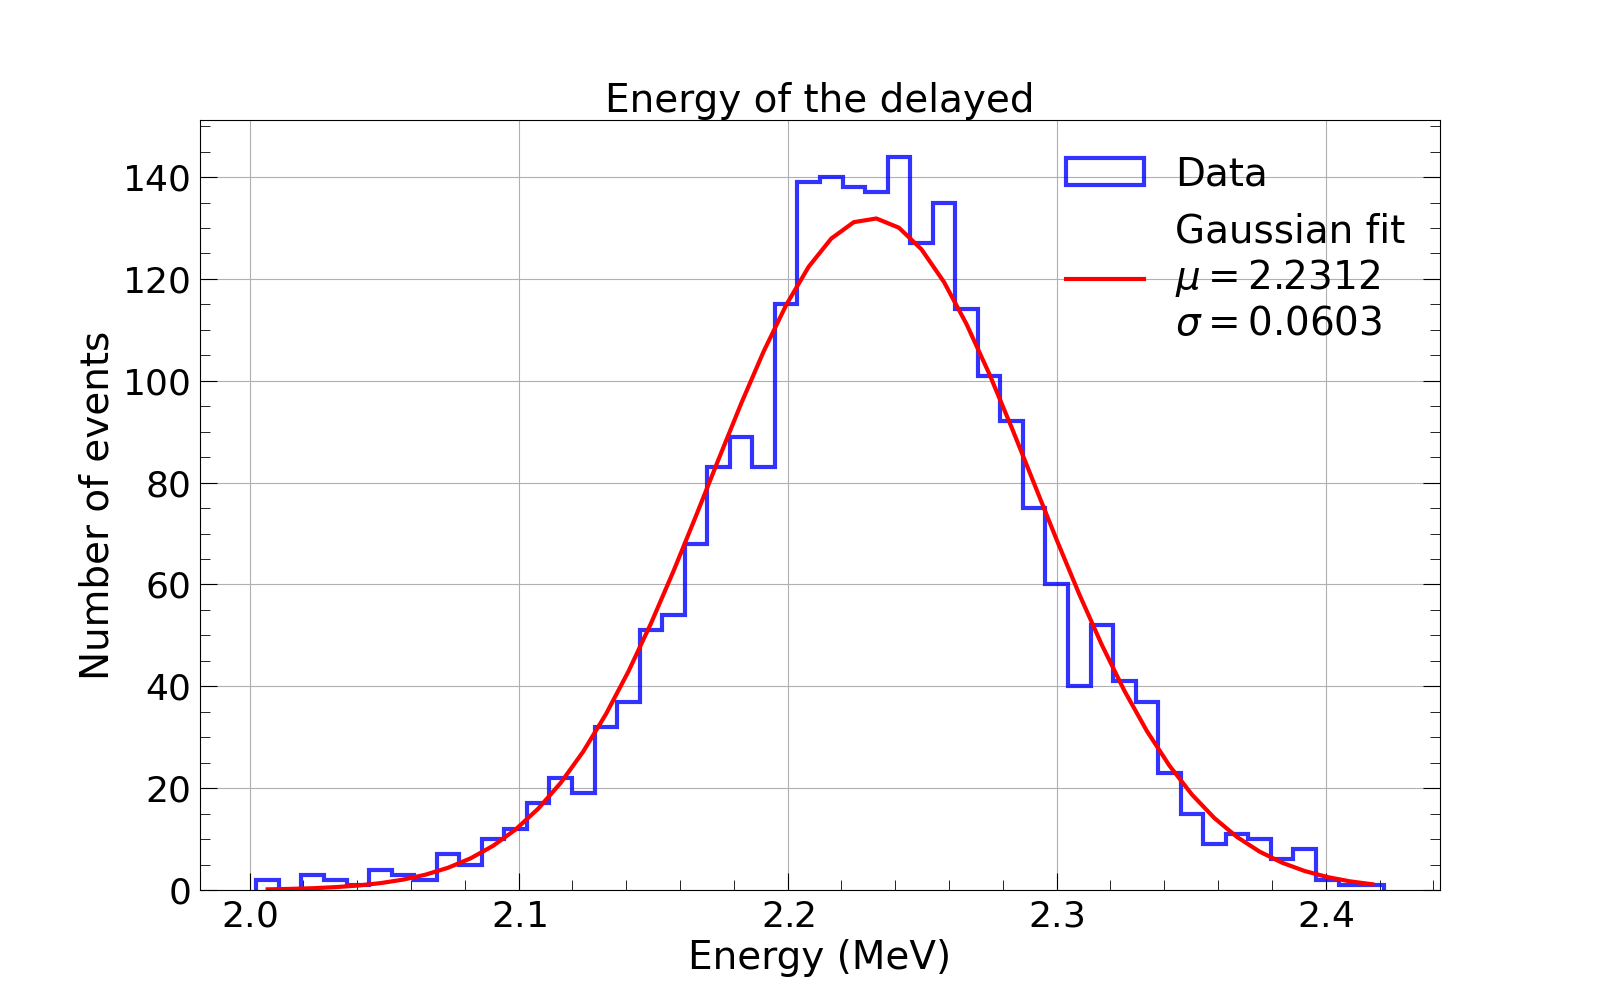
\includegraphics[width=0.49\textwidth]{2_selection/h_ibd_e_d.png}
    \caption{The prompt and delayed energy spectra.}
    \label{fig:IBD_energy_spectra}
\end{figure}


\begin{figure}[!htbp]
    \centering
      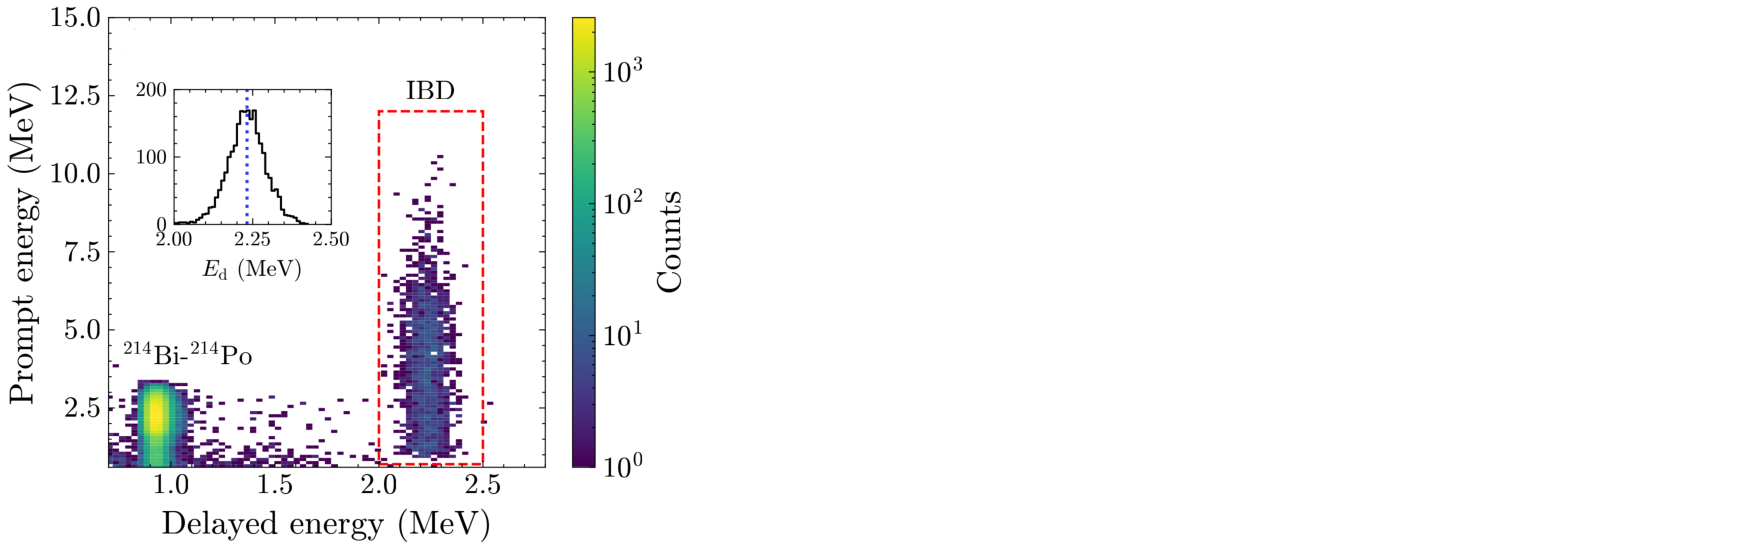
\includegraphics[width=0.7\textwidth]{2_selection/Fig_2D_dt_distance_withgroupABC_noa.pdf}
    \caption{Two-dimensional prompt-versus-delayed energies (with enlarged delayed energy window) showing the $^{214}$Bi-$^{214}$Po cluster at $E_d\sim$1~MeV and the IBD selection region (dashed box).}
    \label{fig:IBD_energy_spectra_2D}
\end{figure}

\begin{figure}[!htbp]
    \centering
    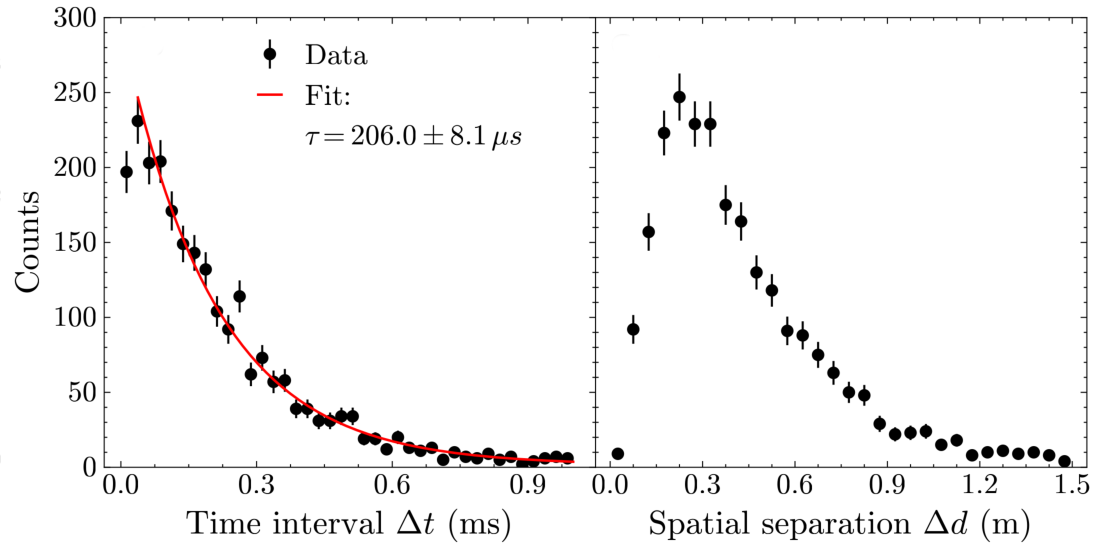
\includegraphics[width=0.8\textwidth]{2_selection/Fig_2D_dt_distance_A.pdf}
    \caption{Left panel: Temporal correlation following an exponential decay with a fitted neutron-capture time of $\tau=206.1\pm8.1\mu s$. The deviation of the first point is due to the $\Delta t >5$~$\mu s$ cut and is therefore not included in the fit. Right panel: Spatial separation $\Delta d$ of the prompt and delayed vertices.}
    \label{fig:IBD_dt}
\end{figure}

\begin{figure}[!htbp]
    \centering
    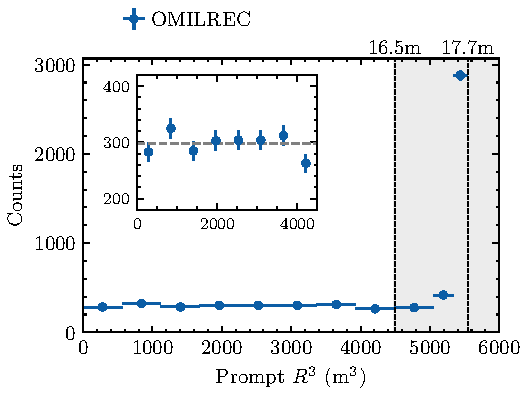
\includegraphics[width=0.8\textwidth]{2_selection/Fig_r3_p_GroupA.pdf}
    \caption{Spatial distribution of reactor neutrino candidates. Prompt-event counts versus reconstructed cubic radius (R3) are shown for the OMILREC. Horizontal bars indicate $R^3$ bin widths; vertical dashed lines mark the FV boundary (16.5 m) and detector edge (17.7 m). The inset shows the uniform event density within the FV, with the dashed line indicating the mean count level. The rising counts beyond the FV are primarily due to accidental coincidences, with minor contributions from fast- and double-neutron backgrounds. }
    \label{fig:IBD_r3}
\end{figure}

\begin{figure}[!htbp]
    \centering
    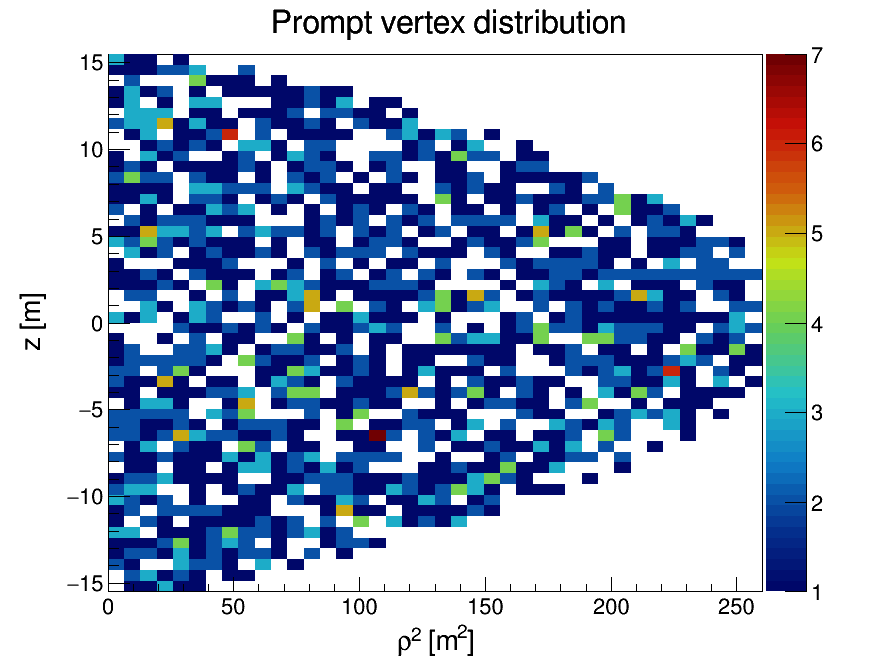
\includegraphics[width=0.49\textwidth]{2_selection/h_ibd_rho_z_p.png}
    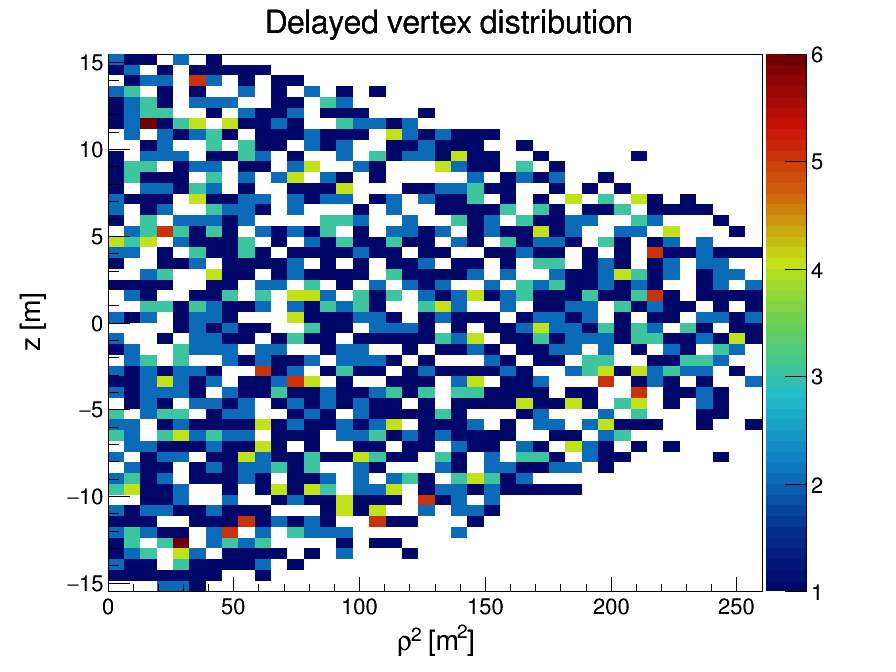
\includegraphics[width=0.49\textwidth]{2_selection/h_ibd_rho_z_d.png}
    \caption{Vertex distribution of the prompt and delayed signals.}
    \label{fig:IBD_vertex}
\end{figure}

\begin{figure}[!htbp]
    \centering
    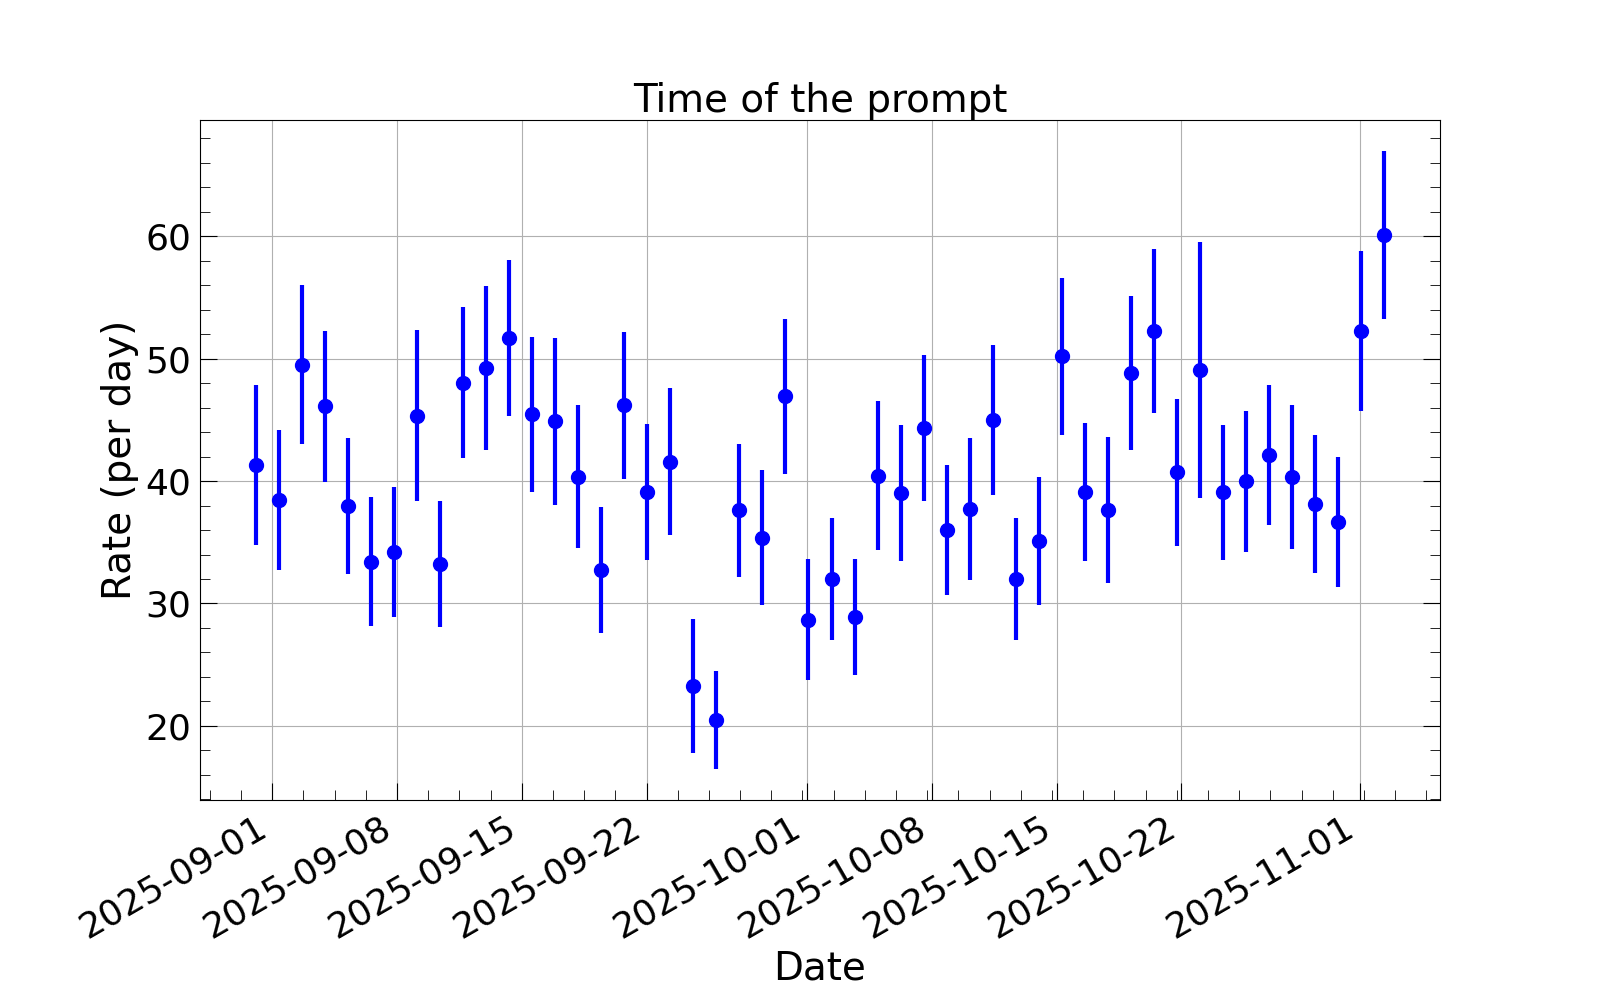
\includegraphics[width=12cm]{2_selection/IBD_rate_reprodb.png}
    \caption{Measured IBD rate as a function of time (no efficiency correction; no background-subtraction).}
    \label{fig:IBDrate}
\end{figure}

%\begin{figure}[!htbp]
%    \centering
%    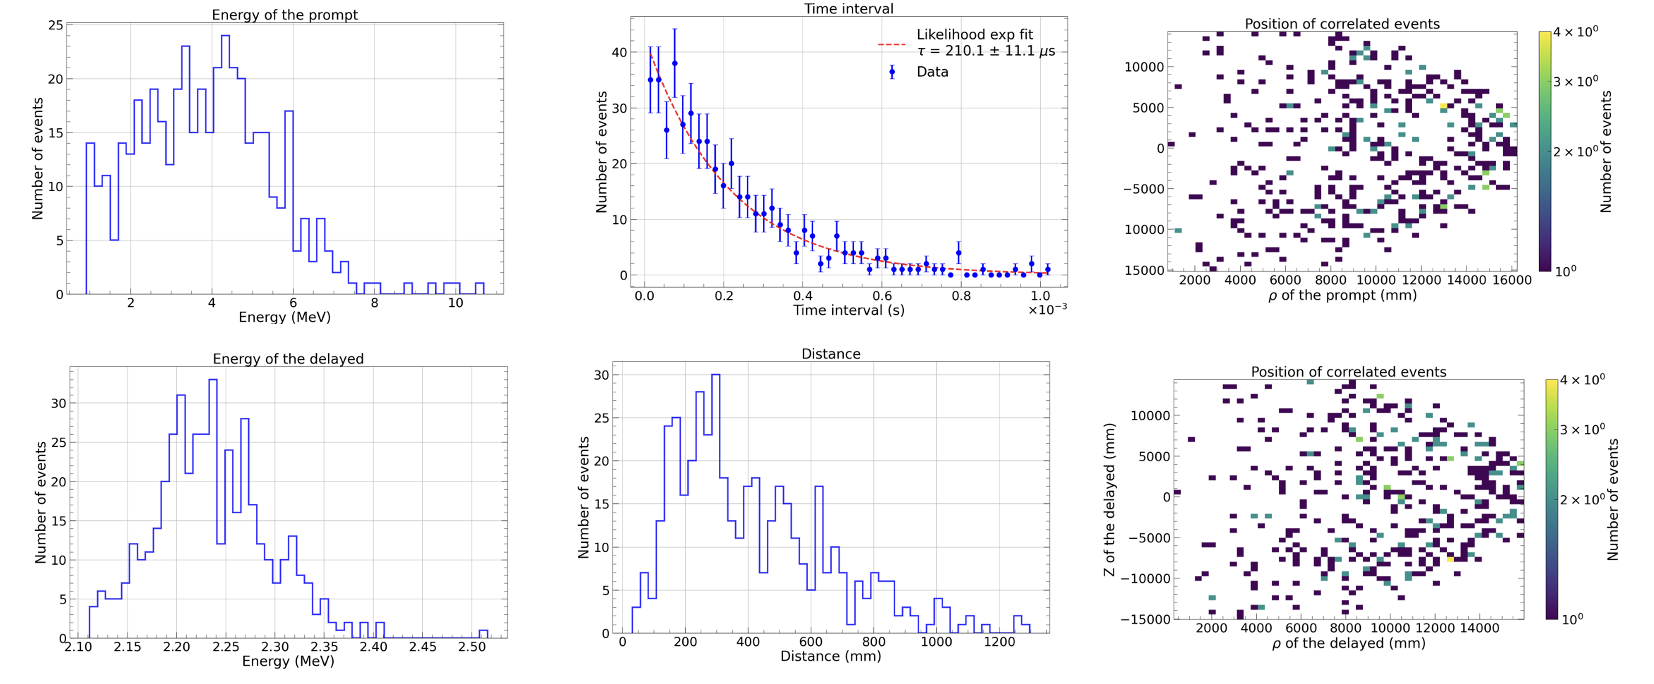
\includegraphics[width=0.9\textwidth]{2_selection/IBD_ReProdA25.png}
%    \caption{IBD distributions using ReProd25A.}
%    \label{fig:IBD_vertex}
%\end{figure}
